\documentclass{standalone}
\usepackage{tikz}
\usetikzlibrary{patterns, positioning}


\begin{document}
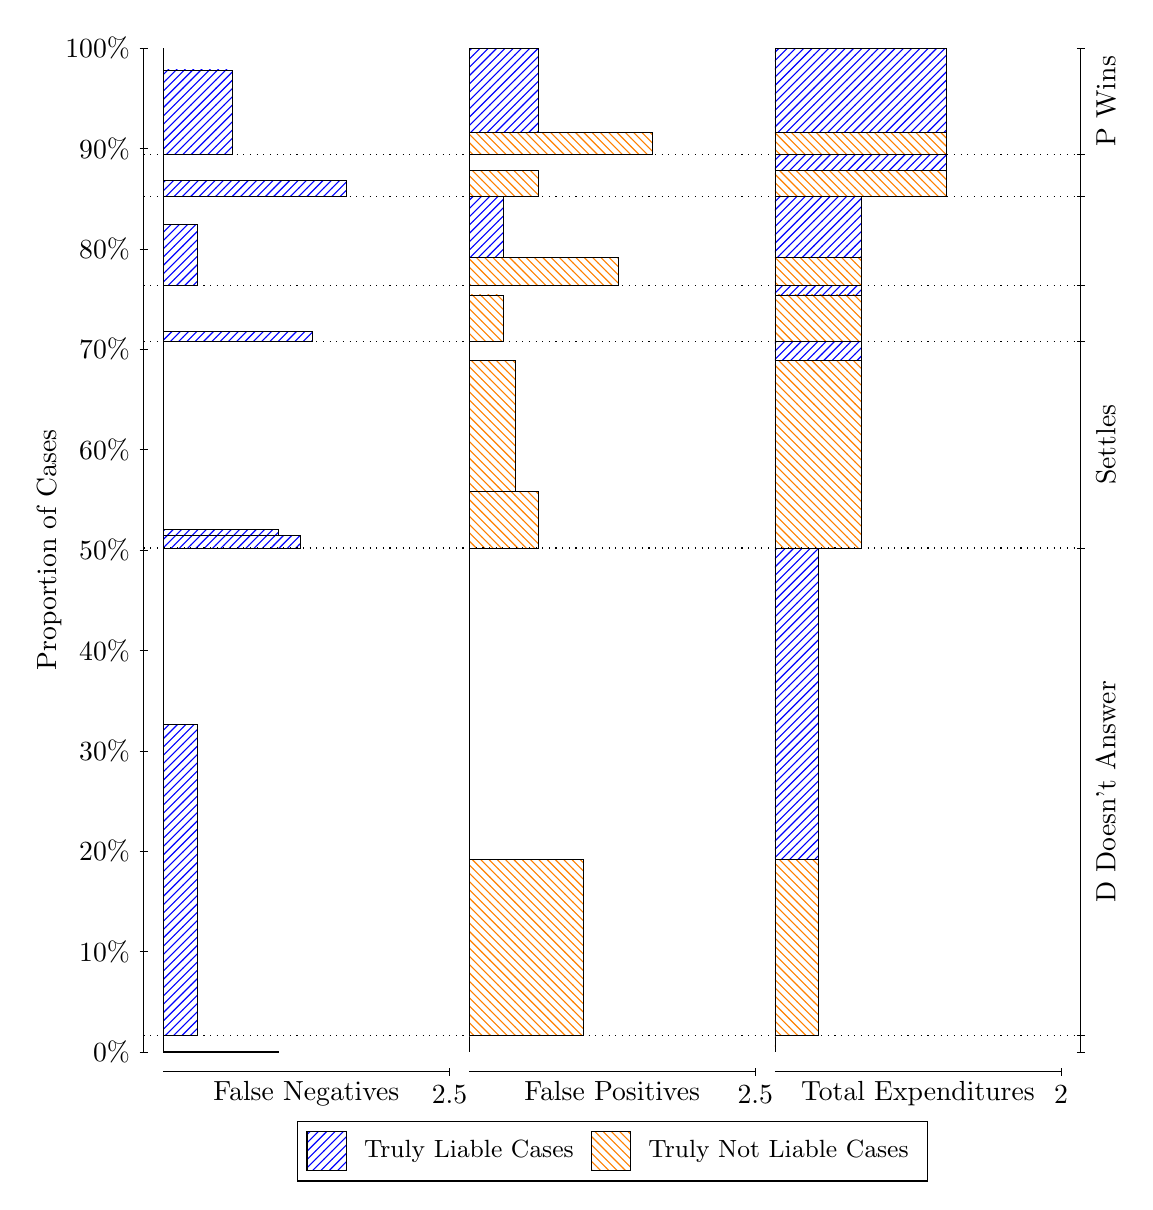
\begin{tikzpicture}
\draw[black, very thin] (1.5,1.75) -- (1.5,14.5);
\node[rotate=90, text=black, anchor=center] at (0.3, 8.125) {Proportion of Cases};
\draw[black, very thin] (1.45,1.75) -- (1.55,1.75);
\node[text=black, anchor=east] at (1.45, 1.75) {0\%};
\draw[black, very thin] (1.45,3.025) -- (1.55,3.025);
\node[text=black, anchor=east] at (1.45, 3.025) {10\%};
\draw[black, very thin] (1.45,4.3) -- (1.55,4.3);
\node[text=black, anchor=east] at (1.45, 4.3) {20\%};
\draw[black, very thin] (1.45,5.575) -- (1.55,5.575);
\node[text=black, anchor=east] at (1.45, 5.575) {30\%};
\draw[black, very thin] (1.45,6.85) -- (1.55,6.85);
\node[text=black, anchor=east] at (1.45, 6.85) {40\%};
\draw[black, very thin] (1.45,8.125) -- (1.55,8.125);
\node[text=black, anchor=east] at (1.45, 8.125) {50\%};
\draw[black, very thin] (1.45,9.4) -- (1.55,9.4);
\node[text=black, anchor=east] at (1.45, 9.4) {60\%};
\draw[black, very thin] (1.45,10.675) -- (1.55,10.675);
\node[text=black, anchor=east] at (1.45, 10.675) {70\%};
\draw[black, very thin] (1.45,11.95) -- (1.55,11.95);
\node[text=black, anchor=east] at (1.45, 11.95) {80\%};
\draw[black, very thin] (1.45,13.225) -- (1.55,13.225);
\node[text=black, anchor=east] at (1.45, 13.225) {90\%};
\draw[black, very thin] (1.45,14.5) -- (1.55,14.5);
\node[text=black, anchor=east] at (1.45, 14.5) {100\%};

\draw[black, very thin] (13.4,1.75) -- (13.4,14.5);
\draw[black, very thin] (13.35,1.75) -- (13.45,1.75);
\node[anchor=west] at (13.35, 1.75) {};
\draw[black, very thin] (13.35,1.9559) -- (13.45,1.9559);
\node[anchor=west] at (13.35, 1.9559) {};
\draw[black, very thin] (13.35,8.1498) -- (13.45,8.1498);
\node[anchor=west] at (13.35, 8.1498) {};
\draw[black, very thin] (13.35,10.775) -- (13.45,10.775);
\node[anchor=west] at (13.35, 10.775) {};
\draw[black, very thin] (13.35,11.487) -- (13.45,11.487);
\node[anchor=west] at (13.35, 11.487) {};
\draw[black, very thin] (13.35,12.611) -- (13.45,12.611);
\node[anchor=west] at (13.35, 12.611) {};
\draw[black, very thin] (13.35,13.148) -- (13.45,13.148);
\node[anchor=west] at (13.35, 13.148) {};
\draw[black, very thin] (13.35,14.5) -- (13.45,14.5);
\node[anchor=west] at (13.35, 14.5) {};

\draw[black, very thin, pattern color=blue, pattern=north east lines] (1.75,1.75) rectangle (3.2033,1.7621);
\draw[black, very thin, pattern color=orange, pattern=north west lines] (1.75,1.7621) rectangle (1.75,1.9559);
\draw[black, very thin, pattern color=blue, pattern=north east lines] (1.75,1.9559) rectangle (2.186,5.9057);
\draw[black, very thin, pattern color=orange, pattern=north west lines] (1.75,5.9057) rectangle (1.75,8.1498);
\draw[black, very thin, pattern color=blue, pattern=north east lines] (1.75,8.1498) rectangle (3.494,8.3077);
\draw[black, very thin, pattern color=blue, pattern=north east lines] (1.75,8.3077) rectangle (3.2033,8.3887);
\draw[black, very thin, pattern color=orange, pattern=north west lines] (1.75,8.3887) rectangle (1.75,10.775);
\draw[black, very thin, pattern color=blue, pattern=north east lines] (1.75,10.775) rectangle (3.6393,10.898);
\draw[black, very thin, pattern color=orange, pattern=north west lines] (1.75,10.898) rectangle (1.75,11.487);
\draw[black, very thin, pattern color=blue, pattern=north east lines] (1.75,11.487) rectangle (2.186,12.262);
\draw[black, very thin, pattern color=orange, pattern=north west lines] (1.75,12.262) rectangle (1.75,12.611);
\draw[black, very thin, pattern color=blue, pattern=north east lines] (1.75,12.611) rectangle (4.0753,12.815);
\draw[black, very thin, pattern color=orange, pattern=north west lines] (1.75,12.815) rectangle (1.75,13.148);
\draw[black, very thin, pattern color=blue, pattern=north east lines] (1.75,13.148) rectangle (2.622,14.222);
\draw[black, very thin, pattern color=orange, pattern=north west lines] (1.75,14.222) rectangle (1.75,14.5);
\draw[black, very thin, pattern color=orange, pattern=north west lines] (5.6333,1.75) rectangle (5.6333,1.9439);
\draw[black, very thin, pattern color=blue, pattern=north east lines] (5.6333,1.9439) rectangle (5.6333,1.9559);
\draw[black, very thin, pattern color=orange, pattern=north west lines] (5.6333,1.9559) rectangle (7.0867,4.2001);
\draw[black, very thin, pattern color=blue, pattern=north east lines] (5.6333,4.2001) rectangle (5.6333,8.1498);
\draw[black, very thin, pattern color=orange, pattern=north west lines] (5.6333,8.1498) rectangle (6.5053,8.8733);
\draw[black, very thin, pattern color=orange, pattern=north west lines] (5.6333,8.8733) rectangle (6.2147,10.536);
\draw[black, very thin, pattern color=blue, pattern=north east lines] (5.6333,10.536) rectangle (5.6333,10.775);
\draw[black, very thin, pattern color=orange, pattern=north west lines] (5.6333,10.775) rectangle (6.0693,11.365);
\draw[black, very thin, pattern color=blue, pattern=north east lines] (5.6333,11.365) rectangle (5.6333,11.487);
\draw[black, very thin, pattern color=orange, pattern=north west lines] (5.6333,11.487) rectangle (7.5227,11.837);
\draw[black, very thin, pattern color=blue, pattern=north east lines] (5.6333,11.837) rectangle (6.0693,12.611);
\draw[black, very thin, pattern color=orange, pattern=north west lines] (5.6333,12.611) rectangle (6.5053,12.944);
\draw[black, very thin, pattern color=blue, pattern=north east lines] (5.6333,12.944) rectangle (5.6333,13.148);
\draw[black, very thin, pattern color=orange, pattern=north west lines] (5.6333,13.148) rectangle (7.9587,13.426);
\draw[black, very thin, pattern color=blue, pattern=north east lines] (5.6333,13.426) rectangle (6.5053,14.5);
\draw[black, very thin, pattern color=orange, pattern=north west lines] (9.5167,1.75) rectangle (9.5167,1.9439);
\draw[black, very thin, pattern color=blue, pattern=north east lines] (9.5167,1.9439) rectangle (9.5167,1.9559);
\draw[black, very thin, pattern color=orange, pattern=north west lines] (9.5167,1.9559) rectangle (10.062,4.2001);
\draw[black, very thin, pattern color=blue, pattern=north east lines] (9.5167,4.2001) rectangle (10.062,8.1498);
\draw[black, very thin, pattern color=orange, pattern=north west lines] (9.5167,8.1498) rectangle (10.607,10.536);
\draw[black, very thin, pattern color=blue, pattern=north east lines] (9.5167,10.536) rectangle (10.607,10.775);
\draw[black, very thin, pattern color=orange, pattern=north west lines] (9.5167,10.775) rectangle (10.607,11.365);
\draw[black, very thin, pattern color=blue, pattern=north east lines] (9.5167,11.365) rectangle (10.607,11.487);
\draw[black, very thin, pattern color=orange, pattern=north west lines] (9.5167,11.487) rectangle (10.607,11.837);
\draw[black, very thin, pattern color=blue, pattern=north east lines] (9.5167,11.837) rectangle (10.607,12.611);
\draw[black, very thin, pattern color=orange, pattern=north west lines] (9.5167,12.611) rectangle (11.697,12.944);
\draw[black, very thin, pattern color=blue, pattern=north east lines] (9.5167,12.944) rectangle (11.697,13.148);
\draw[black, very thin, pattern color=orange, pattern=north west lines] (9.5167,13.148) rectangle (11.697,13.426);
\draw[black, very thin, pattern color=blue, pattern=north east lines] (9.5167,13.426) rectangle (11.697,14.5);
\draw[black, dotted] (1.5,1.9559) -- (13.4,1.9559);
\draw[black, dotted] (1.5,8.1498) -- (13.4,8.1498);
\draw[black, dotted] (1.5,10.775) -- (13.4,10.775);
\draw[black, dotted] (1.5,11.487) -- (13.4,11.487);
\draw[black, dotted] (1.5,12.611) -- (13.4,12.611);
\draw[black, dotted] (1.5,13.148) -- (13.4,13.148);
\draw[black, very thin] (1.75,1.5) -- (5.3833,1.5);
\node[text=black, anchor=north] at (3.5667, 1.5) {False Negatives};
\draw[black, very thin] (5.3833,1.45) -- (5.3833,1.55);
\node[text=black, anchor=north] at (5.3833, 1.45) {2.5};

\draw[black, very thin] (5.6333,1.5) -- (9.2667,1.5);
\node[text=black, anchor=north] at (7.45, 1.5) {False Positives};
\draw[black, very thin] (9.2667,1.45) -- (9.2667,1.55);
\node[text=black, anchor=north] at (9.2667, 1.45) {2.5};

\draw[black, very thin] (9.5167,1.5) -- (13.15,1.5);
\node[text=black, anchor=north] at (11.333, 1.5) {Total Expenditures};
\draw[black, very thin] (13.15,1.45) -- (13.15,1.55);
\node[text=black, anchor=north] at (13.15, 1.45) {2};


\node[text=black, centered, rotate=90] at (13.72, 5.0529) {D Doesn't Answer};
\node[text=black, centered, rotate=90] at (13.72, 9.4626) {Settles};



\node[text=black, centered, rotate=90] at (13.72, 13.824) {P Wins};

\draw (7.449999999999999,1.5) node[draw=none] (baseCoordinate) {};
\begin{scope}[align=center]
        \matrix[scale=0.5, draw=black, below=0.5cm of baseCoordinate, nodes={draw}, column sep=0.1cm]{
            \node[rectangle, draw, minimum width=0.5cm, minimum height=0.5cm, pattern color=blue, pattern=north east lines] {}; &
            \node[draw=none, font=\small, text=black] (B) {Truly Liable Cases}; &
            \node[rectangle, draw, minimum width=0.5cm, minimum height=0.5cm, pattern color=orange, pattern=north west lines] {}; &
            \node[draw=none, font=\small, text=black] (B) {Truly Not Liable Cases}; \\
            };
\end{scope}

\end{tikzpicture}
\end{document}